\section{Integers}
\label{sec:orga8b7d2e}

Integer types refer to numbers without decimal point. There a two kind of
integers, signed and unsigned ones. The type of signed integers starts with the
letter \texttt{i} where unsigned ones start with the letter \texttt{u}.

\begin{center}
  \begin{tabular}{|r|ll|}
    \hline
    size & signed & unsigned\\[0pt]
    \hline
    \hline
    8 & \texttt{i8} & \texttt{u8}\\[0pt]
    16 & \texttt{i16} & \texttt{u16}\\[0pt]
    32 & \texttt{i32} & \texttt{u32}\\[0pt]
    64 & \texttt{i64} & \texttt{u64}\\[0pt]
    arch & \texttt{isize} & \texttt{usize}\\[0pt]
    \hline
  \end{tabular}
\end{center}

The size of the type in bits is written in the type itself, for example
\texttt{i32} is a signed int of 32 bits. The table above presents the list
of integer types implemented in the version 1.0 of ymirc. \texttt{usize} and
\texttt{isize} are architecture dependant and have a size in bits that depends
on the size of the pointers on the targeted system, (i.e. 32 bits on 32 bits
systems, 64 bits on 64 bits system, and so on)


\vspace{-10pt}%
\subsection{Literals}
\label{sec:org2cf045d}

Integer literals can be written using four forms:
\begin{enumerate}
\item octal, starting with \texttt{0o} and containing only numbers ranging from \texttt{0} to \texttt{7}.
  \texttt{0o71217}
  \vspace{-2pt}%
\item hexadecimal, starting with \texttt{0x} and containing numbers ranging from \texttt{0} to \texttt{9} and letters ranging from \texttt{a} to \texttt{f} in lower or upper case.
  \texttt{0xAB87fe}
  \vspace{-2pt}%
\item Binary, starting with \texttt{0b} and containing numbers ranging from \texttt{0} to \texttt{1}. \texttt{0b10010}.
  \vspace{-2pt}%
\item Decimal , starting with nothing special and containing numbers ranging from \texttt{0} to \texttt{9}.
  \texttt{182993}
\end{enumerate}

All four forms can also contain the token \texttt{\_} to separate long integer literal
and make them more readable (i.e. \texttt{1\_000\_000\_000}). There can be as many \texttt{\_} as
wanted, there are just removed during the compilation.

Literal have to end with a suffix to define a literal from another int type than
\texttt{i32}. For example to define a literal of value \texttt{67} and of type \texttt{i8}, the
following has to be written \texttt{67i8} or \texttt{0x43i8} or \texttt{0o103i8}. A verification is
made during the compilation to ensure that the selected int type has enough
bytes to encode the expected literal. Suffixes for \texttt{isize} and \texttt{usize} are
respectively \texttt{is} and \texttt{us}.

\subsection{Properties}
\label{sec:orgc02cb40}

Integer properties are accessed using the operator \texttt{::} (as for any type) on a type expression. The properties are the following:

\begin{center}
  \vspace{-3pt}
  \begin{adjustbox}{max width=\linewidth}
    \begin{tabular}{|l|ll|}
      \hline
      name & value & type\\[0pt]
      \hline
      \hline
      \texttt{init} & The initial value \texttt{0} & \texttt{typeof(x)}\\[0pt]
      \texttt{max} & The maximum value the type can encode & \texttt{typeof(x)}\\[0pt]
      \texttt{min} & The minimum value the type can encode & \texttt{typeof(x)}\\[0pt]
      \hline
      \texttt{typeid} & A string encoding the name of the type & \texttt{[c8]}\\[0pt]
      \hline
    \end{tabular}
  \end{adjustbox}
\end{center}

\smallskip

Example:
\smallskip

\begin{lstlisting}[style=coloredverbatim]
  println (i32::max); // 2_147_483_647
  println (i16::min); // -32_768
\end{lstlisting}

\subsection{Casting}
\label{sec:orgfdc3d25}

\begin{itemize}
\item To other integers: It is impossible to change the type of an int value implicitely meaning it is
  impossible to transform a value of type \texttt{i32} to value of type \texttt{i64} without
  specifically mentionning it. The cast operator \texttt{cast!T (V)} can transform any int
  type to another int type.

  There is one exception to the previous rule. If a literal value is written
  without suffix, it can be transformed into a value of any int type as long as
  it is known at compilation time. Overflow checking is performed to ensure the
  casting is possible. For example, the following is allowed:

  \begin{lstlisting}[style=coloredverbatim]
def foo (a : u64) { // ... }

let a : i64 = 1;
foo (7 + a); // 7 + a can be known at compilation time, 'a' is immutable and cte
  \end{lstlisting}

\item To char types: The cast operator can be used to transform a int type of type \texttt{u8} into a
  \texttt{c8}, a \texttt{u32} to a \texttt{c32} and a \texttt{u16} into a \texttt{c16} and converserly (e.g. \texttt{c8} to \texttt{u8}). That is the only allowed casting from int to chars. No implicit
  casting is allowed. The transformation does not modify the value in any way
  (exactly the same bits before and after the cast).
  \begin{lstlisting}[style=coloredverbatim]
let a : c32 = cast!c32 (97u32);
let b : u8 = cast!u8 ('a'c8);
  \end{lstlisting}

\item To float types: The casting to floating point types is allowed from any int type whose type
  has a size of at least \texttt{4} bytes (\texttt{i32}, \texttt{u32} and higher) to any floating
  point type, and converserly using the cast operator. This is the only allowed
  casting from int to float types. No implicit casting is allowed. The value
  encoding is modified to be correctly represented. Indeed, int and float have
  completely different ways of representing types in memory. The value is
  truncated when transformed from a float to an int. And there may be some
  stepping when transforming an int value into a float values due to the holes
  present in the set of values representable by float encoding system.

  \begin{lstlisting}[style=coloredverbatim]
let a : f32 = cast!f32 (97u32);
let b : f64 = cast!f64 (12);

let c : i64 = cast!i64 (67.87);
  \end{lstlisting}

\end{itemize}

\subsection{Unary operators}
\label{sec:orge691bb5}

The following unary operators can be used on int types.
\smallskip


%% \begin{adjustbox}{max width=\linewidth}
\begin{center}
  \vspace{-5pt}
  \begin{threeparttable}
    \begin{tabular}{|l|ll|}
      \hline
      Operator & Operation & Example\\[0pt]
      \hline
      \hline
      \texttt{-} & Opposite value & \texttt{-19}\\[0pt]
      \hline
      \texttt{!} & Byte Not\(^{1}\) & \texttt{!19 == -20}\\[0pt]
      \hline
    \end{tabular}
    \begin{tablenotes}

    \item[1.] \footnotesize \textit{inverts each bit from the binary representation of the int value. This is semantically the same as calculating \texttt{-x-1} (if the integer is signed)}

    \end{tablenotes}
  \end{threeparttable}
\end{center}
%% \end{adjustbox}

The result of unary operations always has the same type as the operand used in the operation. Opposite operator \texttt{-} is not usable on unsigned type, as they cannot be negative.


\subsection{Binary operators}
\label{sec:orgb91194f}

Binary operators involving an int operand can only be used when the two operands
are of type int. There are two exception to that rule 1. When the operation
involves an object operand that has overriden the said binary operator (as left
or right operand), 2. When on of the operand is a char type or a pointer type.
Binary operators involving char types are presented in the section about char
types, and involving pointer types are presented in the chapter about compound
types.

Binary operators are divided into 5 groups:
\begin{itemize}
\item Math: Binary math operators are usable using two int values whose types
  have the same signed property (two signed operands or two unsigned operands,
  but not a mix). The result of the operation takes the type of the biggest of
  the two operands for example for an addition between a \texttt{i64} and a
  \texttt{i32} (e.g. \texttt{12 + 78i64}), the result takes the type
  \texttt{i64}. There is an exception, being the exponant operator, where the
  right operand is always a \texttt{i32}, and the results always takes the type
  of the left operand.


  \begin{center}
    \vspace{-10pt}
    \begin{adjustbox}{max width=1.0\linewidth}
      \begin{tabular}{|c|lll|}
        \hline
        Operator & Operation & Commutative & Example\\[0pt]
        \hline
        \hline
        \texttt{+} & Addition & Yes & \texttt{1 + 2 == 3}\\[0pt]
        \texttt{-} & Subtraction & No & \texttt{2 - 1 == 1}\\[0pt]
        \texttt{*} & Multiplication & Yes & \texttt{3 * 4 == 12}\\[0pt]
        \texttt{/} & Division (truncate) & No & \texttt{13 / 3 == 4}\\[0pt]
        \texttt{\%} & Rest of the division & No & \texttt{13 \% 3 == 1}\\[0pt]
        \texttt{\textasciicircum{}\textasciicircum{}} & Exponant & No & \texttt{3\textasciicircum{}\textasciicircum{}4 == 81}\\[0pt]
        \hline
      \end{tabular}
    \end{adjustbox}
  \end{center}

\item Bytes: Bytes binary operators are usable using two int values having
  exactly the same type (e.g. \texttt{i64} with and only with \texttt{i64}).

  \begin{center}
    \vspace{-20pt}
    \begin{adjustbox}{max width=1.0\linewidth}
      \begin{tabular}{|c|l l l|}
        \hline
        Operator & Operation & Commutative & Example \\[0pt]
        \hline
        \hline
        \texttt{\(\vert\)} & Byte Or & Yes & \texttt{0b001} \(\vert{}\) \texttt{0b010 == 0b011}\\[0pt]
        \texttt{\&} & Byte And & Yes & \texttt{0b001 \& 0b010 == 0b000}\\[0pt]
        \texttt{\textasciicircum{}} & Byte Xor & Yes & \texttt{0b001 \textasciicircum{} 0b011 == 0b010}\\[0pt]
        \texttt{>>} & Byte left shift & No & \texttt{0b100000 >> 0b010 == 0b001000}\\[0pt]
        \texttt{<<} & Byte right shift & No & \texttt{0b001000 << 0b010 == 0b100000}\\[0pt]
        \hline
      \end{tabular}
    \end{adjustbox}
  \end{center}

\item Logical: Binary logical operators are usable using two int values whose
  types have the same signed property (two signed operands or two unsigned
  operands, but not a mix). The biggest type of the two integers is used to cast
  the value of the operand with the smallest type. The result of the operation
  always takes the type \texttt{bool}.

  \begin{center}
    \vspace{-20pt}
    \begin{adjustbox}{max width=1.0\linewidth}
      \begin{tabular}{|c|l l l|}
        \hline
        Operator & Operation & Commutative & Example\\[0pt]
        \hline
        \hline
        \texttt{>} & Greater than & No & \texttt{(12 > 11) == true}\\[0pt]
        \texttt{<} & Lower than & No & \texttt{(12 < 11) == false}\\[0pt]
        \texttt{>=} & Greater or equal & No & \texttt{(14 >= 14) == true}\\[0pt]
        \texttt{<=} & Lower or equal & No & \texttt{(11 <= 19) == true}\\[0pt]
        \texttt{==} & Equal & Yes & \texttt{(10 == 10) == true}\\[0pt]
        \texttt{!=} & Not equal & Yes & \texttt{(10 != 10) == false}\\[0pt]
        \hline
      \end{tabular}
    \end{adjustbox}
  \end{center}

\item Affectation: The affectation operator \texttt{=} is usable when the two
  operands have strictly the same int type. The left operand must be a mutable
  lvalue (e.g. a mutable variable, a slice access, etc.). Affectation operator
  can be mixed with a math or byte operator (e.g. \texttt{+=}, \texttt{\&=},
  etc.). In that case the operation \texttt{x += y} is rewritten into \texttt{x
    = x + (y)}, where the y operand has always higher priority than the
  affectation operator. For example the operation \texttt{x *= 12 + 3} will be
  rewritten into \texttt{x = x * (12 + 3)} even though the multiplication
  operator has a higher priority than the addition operator, meaning that the
  result of \texttt{x *= (12 + 3)} is different to the result of \texttt{x = (x
    * 12 + 3)}.

  \begin{lstlisting}[style=coloredverbatim]
let mut a = 11;
let b = a * 12 + 3;
a *= 12 + 3;

assert (b == 135);
assert (a == 165);
  \end{lstlisting}

\item Range: The range operator can be used on int values of strictly the same type,
  creating a \texttt{range} value. The range type is a native compound type that is
  described in the next chapter.

  \begin{center}
    \vspace{-20pt}
    \begin{adjustbox}{max width=1.0\linewidth}
      \begin{tabular}{|c|lll|}
        \hline
        Operator & Operation & Example & Interval\\[0pt]
        \hline
        \texttt{..} & Range operator not inclusive & \texttt{34 .. 12} & \texttt{[34;12[}\\[0pt]
            \texttt{...} & Range operator inclusive & \texttt{5 ... 89} & \texttt{[5;89]}\\[0pt]
            \hline
      \end{tabular}
    \end{adjustbox}
  \end{center}

  The result range value has a default step of \texttt{1} and its inner type is the type
  of the operand. It can be increasing or decreasing depending on the values
  used to construct it.

\end{itemize}

\subsection{Overflowing}
\label{sec:org0881da2}

Compile time verification of value overflowing is made on cte values. There is
no way to check an overflow at runtime, and it may occur.

\begin{figure*}[t]
  \centering
  \scalebox{0.9}{
    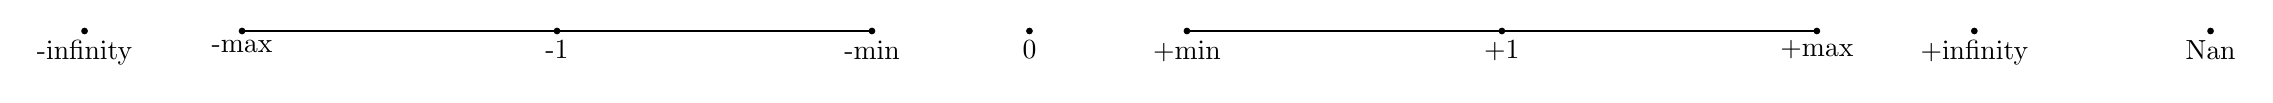
\begin{tikzpicture}
      \filldraw (0,0) circle (1pt) node[align=center, below] {-infinity};
      \filldraw (2,0) circle (1pt) node[align=center, below] {-max};
      \filldraw (6,0) circle (1pt) node[align=center, below] {-1};
      \filldraw (10,0) circle (1pt) node[align=center, below] {-min};
      \filldraw (12,0) circle (1pt) node[align=center, below] {0};
      \filldraw (14,0) circle (1pt) node[align=center, below] {+min};
      \filldraw (18,0) circle (1pt) node[align=center, below] {+1};
      \filldraw (22,0) circle (1pt) node[align=center, below] {+max};
      \filldraw (24,0) circle (1pt) node[align=center, below] {+infinity};
      \filldraw (27,0) circle (1pt) node[align=center, below] {Nan};

      \draw[-](2,0) -- (10, 0);
      \draw[-](14,0) -- (22, 0);

    \end{tikzpicture}
  }
  \caption{\label{float_point_size} Range of representable values with floating point types}
\end{figure*}


\section{Floating point types}
\label{sec:orgae6ed5f}

Floating point types refer to numbers with a decimal point. There are 4
floating, presented in the table below. Builtin floating point types conform to
the IEEE 754 arithmetic, meaning for example that \texttt{f32} have 1 bit of sign, \texttt{8}
bits of exponent, and \texttt{24} (23 explicit) bits of mantissa. \texttt{fsize} type represent
the biggest floating point type that can be represented on the target
architecture.

\begin{center}
  \vspace{-5pt}
  \begin{tabular}{|c|lll|}
    \hline
    type & size & exp & mantissa\\[0pt]
    \hline
    \hline
    \texttt{f32} & 32 & 8 & 24 (23 explicit)\\[0pt]
    \texttt{f64} & 64 & 11 & 53 (52 explicit)\\[0pt]
    \texttt{f80} & 80 & 16 & 64 (63 explicit)\\[0pt]
    \texttt{fsize} & arch & arch & arch\\[0pt]
    \hline
  \end{tabular}
\end{center}




\subsection{Literals}
\label{sec:orgfd9f825}

Floating point types can be written using three different forms, decimal, scientific notation.
\begin{enumerate}
\item Decimal, two decimal int literals seperated with the token \texttt{.} (with no
  white space in between). \texttt{1837.0289}. The decimal part can be omitted
  meaning it is equal to \texttt{0} (e.g. \texttt{10.} is valid, but not \texttt{.10}).

\item Scientific notation, same as decimal notation but ending with an exponent
  preceded by the letter \texttt{e} or \texttt{E}. \texttt{3.14e78 == (3.14 * 10.0 \textasciicircum{}\textasciicircum{} 78)}, meaning
  \(3.14 \times 10^{78}\). A signed can be set for exponential part following the
  letter \texttt{e} or \texttt{E} with the token \texttt{-} or \texttt{+}, e.g. \texttt{3.e-10}. There cannot be
  any space in the literal.

\item Hexadecimal notation, starting with \texttt{0x}, then two hexadecimal int literal
  separated with the token \texttt{.} followed by the letter \texttt{p} or \texttt{P}, and finishing
  with a decimal int literal representing the exponential part. The fraction
  part can be empty, in that case the letter \texttt{p} follows the \texttt{.} token.
  However, the \texttt{.} token and the exponential part \texttt{p} are mandatory. A sign can
  be set for exponential part following the letter \texttt{p} or \texttt{P} with the token
  \texttt{-} or \texttt{+}. There cannot be any space in the literal. Unlike scientific
  notation, the exponential part is a power of \texttt{2} instead of \texttt{10}, e.g.
  \texttt{0xA.p4 == (10.0 * 2.0\textasciicircum{}\textasciicircum{}4)}.
\end{enumerate}

The three forms can also include the token \texttt{\_} to separate long literals and
make them easier to read (e.g. \texttt{124\_732.789\_281}, \texttt{0x1.FFFF\_FFFFp1023},
\texttt{3.14\_15\_92e3f}). There can be as many \texttt{\_} as wanted, there are just removed
during the compilation. Literals can end with a suffix to specify the type of the
literal; \texttt{f} to define \texttt{f32} literals, \texttt{d} to define \texttt{f64} (for \texttt{double}), \texttt{l}
for \texttt{f80} (for \texttt{long}) and \texttt{r} for \texttt{fsize} (for \texttt{real}). Literals with no suffix
are considered of type \texttt{f64}. The literal \texttt{4.5e10f} and \texttt{0.8f}, \texttt{0x1.FFp10f} are
of type \texttt{f32} when \texttt{4.5e10} and \texttt{0.8}, \texttt{0x1.FFp10} are of type \texttt{f64}.

\subsection{Properties}
\label{sec:org52a5d6e}

Floating point properties are accessible using the operator \texttt{::} on a
type expression. The properties are the following:

\begin{center}
  \vspace{-5pt}
  \begin{adjustbox}{max width=1.01\linewidth}
    \begin{threeparttable}
      \begin{tabular}{|l|ll|}
        \hline
        Name & Meaning & Type\\[0pt]
        \hline
        \hline
        \texttt{init} & The initial value - nan (Not a Number) & \texttt{typeof(x)}\\[0pt]
        \Xhline{0.001pt}
        \texttt{max} & The maximal finite value & \texttt{typeof(x)}\\
        & that this type can encode & \\[0pt]
        \Xhline{0.001pt}

        \texttt{min} & The minimal finite value & \texttt{typeof(x)}\\
        & that this type can encode & \\[0pt]
        \Xhline{0.001pt}

        \texttt{nan} & The value Not a Number & \texttt{typeof(x)}\\[0pt]
        \Xhline{0.001pt}
        \texttt{inf} & The value positive infinity & \texttt{typeof(x)}\\[0pt]
        \Xhline{0.001pt}
        \texttt{epsilon} & The smallest increment & \texttt{typeof(x)}\\
        & to the value 1 &\\[0pt]
        \Xhline{0.001pt}
        \texttt{dig} & The number of decimal digit of precision & \texttt{u32}\\[0pt]
        \Xhline{0.001pt}
        \texttt{mant\_dig} & Number of bits in the mantissa & \texttt{u32}\\[0pt]
        \Xhline{0.001pt}
        \texttt{max\_10\_exp} & The maximum value &  \texttt{i32} \\
        & such that \(10^{max\_10\_exp}\) is representable &\\[0pt]
        \Xhline{0.001pt}
        \texttt{max\_exp} & The maximum value & \texttt{i32}\\
        & such that \(2^{max\_exp-1}\) is representable & \\[0pt]
        \Xhline{0.001pt}
        \texttt{min\_10\_exp} & The minimum value & \texttt{i32}\\
        & such that \(10^{min\_10\_exp}\) is representable$^1$  & \\[0pt]
        \Xhline{0.001pt}
        \texttt{min\_exp} & The minimum value & \texttt{i32}\\
        & such that \(2^{min\_exp-1}\) is representable$^1$ & \\[0pt]
        \hline
        \texttt{typeid} & A string encoding the name of the type & \texttt{[c8]}\\[0pt]
        \hline
      \end{tabular}
      \begin{tablenotes}
      \item[1.] \small \textit{as a normalized value}
      \end{tablenotes}
    \end{threeparttable}
  \end{adjustbox}
\end{center}

\smallskip

The \texttt{min} value is not the opposite value of the \texttt{max} value. The
Figure~\ref{float_point_size} describes the order relation between values of
floating point types, where points and lines are the values that are
representable by a floating point type.


\subsection{Casting}
\label{sec:org9eacb07}

\begin{itemize}
\item To other floating point types: It is impossible to change the type of a float value implicitely. The cast
  operator \texttt{cast!T (V)} can transform any float type into another float type.

\item To integer types: The cast operator can be used to transform a float value of any float type
  into a int value whose type has a size of at least 4 bytes (\texttt{i32}, \texttt{u32} and
  bigger). When using the cast operator, the value is truncated to the floor
  value (e.g. \texttt{1.3} \texttt{1.5} and \texttt{1.8} are all truncated to \texttt{1}), and everything
  that were part of the decimal part of the float value is lost. The opposite
  cast is also allowed (from any int type whose size is at least \texttt{4} bytes to
  any float type); in that case some stepping can occur due to floating point
  encoding.
\end{itemize}

Floating point types cannot be transformed into other types.

\subsection{Unary operators}
\label{sec:org30770bf}

The \texttt{-} unary operators can be used on floating point types. The result of the
operation is the opposite value, and has the same type as the operand of the
operation. For example \texttt{-89.0f} is of type \texttt{f32}.

\subsection{Binary operators}
\label{sec:orga43d13a}

Binary operators involving a float operand can be used only when the two
operands are floats. There is an exception to that rule when the operation
involves an object operand that has overriden the said binary operator (for left
or right operand). Binary operators are divided into 4 groups:
\begin{itemize}
\item Math: Binary math operators are usable using two float values. The result of the
  operation takes the type of the biggest operand (e.g. operation with \texttt{f32} and
  \texttt{f64} takes the type \texttt{f64}).  Usable operators are described in the
  following table.

  \begin{center}
    \vspace{-20pt}
    \begin{adjustbox}{max width=1.0\linewidth}
      \begin{tabular}{|c|lll|}
        \hline
        Operator & Operation & Commutative & Example\\[0pt]
        \hline
        \hline
        \texttt{+} & Addition & Yes & \texttt{1.0 + 2.3 == 3.3}\\[0pt]
        \texttt{-} & Subtraction & No & \texttt{1. - 8. == -7.}\\[0pt]
        \texttt{*} & Multiplication & Yes & \texttt{3. * 4. == 12.}\\[0pt]
        \texttt{/} & Division & No & \texttt{7. / 3. == 2.333}\\[0pt]
        \texttt{\%} & Rest of division & No & \texttt{7.23 \% 3.09 == 1.05}\\[0pt]
        \texttt{\textasciicircum{}\textasciicircum{}} & Exponant & No & \texttt{7. \textasciicircum{}\textasciicircum{} 3 == 343.}\\[0pt]
        \hline
      \end{tabular}
    \end{adjustbox}
  \end{center}

  Power operator \texttt{\textasciicircum{}\textasciicircum{}} is a special operator that can take a float or an integer
  value as right operand. If both operands are float values, then they must
  share the exact same type, and result value takes the type of the operands. If
  the right operand is an int value, then the result of the operation takes the
  type of the left operand.

\item Logical: Binary logical operators are usable using two float values. The biggest type
  of the two operands is used to cast the value of the operand with the smallest
  type. The result of the operation always takes the type \texttt{bool}.

  \begin{center}
    \vspace{-20pt}
    \begin{adjustbox}{max width=1.0\linewidth}
      \begin{tabular}{|c|lll|}
        \hline
        Operator & Operation & Commutative & Example\\[0pt]
        \hline
        \hline
        \texttt{>} & Greater than & No & \texttt{(12 > 11) == true}\\[0pt]
        \texttt{<} & Lower than & No & \texttt{(12 < 11) == false}\\[0pt]
        \texttt{>=} & Greater or equal & No & \texttt{(14 >= 14) == true}\\[0pt]
        \texttt{<=} & Lower or equal & No & \texttt{(11 <= 19) == true}\\[0pt]
        \texttt{==} & Equal & Yes & \texttt{(10 == 10) == true}\\[0pt]
        \texttt{!=} & Not equal & Yes & \texttt{10 != 10) == false}\\[0pt]
        \hline
      \end{tabular}
    \end{adjustbox}
  \end{center}

\item Affectation: The affectation operator \texttt{=} is usable when the two operands have strictly the
  same float type. The left operand must be a mutable lvalue (e.g. a mutable
  variable, a slice access, etc.). Affectation operator can be mixed with a math
  operator (e.g. \texttt{+=}, \texttt{/=}, etc.). In that case the operation \texttt{x += y}
  is rewritten into \texttt{x = x + (y)}, where the y operand has always higher
  priority than the affectation operator. For example the operation \texttt{x *= 12. +
    3.} will be rewritten into \texttt{x = x * (12. + 3.)} even though the multiplication
  operator has a higher priority than the addition operator, meaning that the
  result of \texttt{x *= (12. + 3.)} is different to the result of \texttt{x = (x * 12. + 3.)}.

  \begin{lstlisting}[style=coloredverbatim]
    let mut a = 11.0;
    let b = a * 12.0 + 3.0;
    a *= 12.0 + 3.0;

    assert (b == 135.0);
    assert (a == 165.0);
  \end{lstlisting}

\item Range: The range operator can be used on two float values of strictly the
  same type, creating a \texttt{range} value. The range type is a native
  compound type that is described in this chapter.

  \begin{center}
    \vspace{-20pt}
    \begin{adjustbox}{max width=1.0\linewidth}
      \begin{tabular}{|l|lll|}
        \hline
        Operator & Operation & Example & Interval\\[0pt]
        \hline
        \hline
        \texttt{..} & Range operator not inclusive & \texttt{34.f .. 12.f} & \texttt{[34.f;12.f[}\\[0pt]
            \texttt{...} & Range operator inclusive & \texttt{5.f ... 89.f} & \texttt{[5.f;89.f]}\\[0pt]
            \hline
      \end{tabular}
    \end{adjustbox}
  \end{center}


  The result range value has a default step of \texttt{1.0} and its inner type is the
  type of the operand. It can be increasing or decreasing depending on the
  values used to construct it.

\end{itemize}

\subsection{Overflowing and stepping}
\label{sec:orgd5d9f51}

Because of the encoding of the float values, holes are presents in the set of
values they can represent. Thus, some operation that should be mathematically
equivalent do not always produce the same float value. To compare two float
values the property \texttt{::epsilon} can be used. There is no check neither at
compile time nor at runtime for value overflowing.


\section{Bool}
\label{sec:org9f3a743}

Bool type is a simple type that can describe only two values \texttt{true} and \texttt{false}.

\subsection{Properties}
\label{sec:org503bc9e}

Properties of \texttt{bool} type are accessible using the operator \texttt{::} on a type
expression. The properties are the following:

\begin{center}
  \vspace{-5pt}
  \begin{adjustbox}{max width=\linewidth}
    \begin{tabular}{|l|ll|}
      \hline
      Name & Meaning & Type\\[0pt]
      \hline
      \hline
      \texttt{init} & The initial value \texttt{false} & \texttt{bool}\\[0pt]
      \hline
      \texttt{typeid} & A string encoding the name of the type & \texttt{[c8]}\\[0pt]
      \hline
    \end{tabular}
  \end{adjustbox}
\end{center}

\subsection{Literals}
\label{sec:org7620b9c}

Boolean literals are the keywords \texttt{true} and \texttt{false}.

\subsection{Casting}
\label{sec:org7cd1f94}

The \texttt{bool} type can be cast using the cast operator to the type \texttt{u8}. This is
the only cast allowed for boolean type. It is impossible to transform a bool
value into a value of another type without explicitely using the cast operator.

\subsection{Unary operators}
\label{sec:orgb412ce4}

The unary operator \texttt{!} can be used on a boolean value to get its opposite value,
(i.e. \texttt{!true} becoming \texttt{false} and \texttt{!false} becoming \texttt{true}).

\subsection{Binary operators}
\label{sec:org030ae50}

Binary operators involving bool operand can only be used if the two operands are
bool of type bool. There is an exception to that rule when the operation
involves an object operand that has overriden the said operator (as left or
right operand).

Binary operators are divided into 3 groups:
\begin{itemize}
\item Affectation: Affectation operators can be used to change the value of a mutable lvalue of
  type bool using a right operand of type bool. Because there are no math
  operators usable on a bool values, no math operator can be attached to the
  affectation operation. \texttt{\&\&=} and \texttt{||=} are not valid operators, and their usage
  will result in a syntax error.

\item Comparison: The comparison \texttt{==} and \texttt{!=} are usable using
  two bool values, to respectively evaluate equality and inequality.

\item Logical: logical operators are usable with two bool operands.

  \begin{center}
    \vspace{-20pt}
    \begin{adjustbox}{max width=1.0\linewidth}
      \begin{tabular}{|c|l l l|}
        \hline
        Operator & Operation & Commutative & Example\\[0pt]
        \hline
        \hline
        \texttt{\(\vert\vert\)} & Or & No & \texttt{false} \(\vert{} \vert{}\) \texttt{true == true}\\[0pt]
        \texttt{\&\&} & And & No & \texttt{true \&\& false == false}\\[0pt]
        \hline
      \end{tabular}
    \end{adjustbox}
  \end{center}

  Operator \texttt{\&\&} and \texttt{||} are marked not commutative. It is not because they can
  return a different value if left and right operands are reverted, but because
  for \texttt{\&\&}, right operand is not evaluated if the left operand is false, and for
  \texttt{||}, right operand is not evaluated if left operand is true. It can be useful
  when chaining tests.

  \begin{lstlisting}[style=coloredverbatim]
let i = 12;
let p = &i;

// if 'p is null', '*p == 12' is not evaluated
let a = p !is null && *p == 12;

// if 'p is null', '*p != 12' is not evaluated
let b = p is null || *p != 12;

// foo function is not called
let c = true || foo ();

// foo function is called
let d = false || foo ();
  \end{lstlisting}
\end{itemize}

\section{Characters}
\label{sec:org344e87e}

Character types are used to encode characters (ascii, or unicode). There are
three char types \texttt{c8}, \texttt{c16} and \texttt{c32} with a respective size of \texttt{8}, \texttt{16} and
\texttt{32} bits. Those char types are encoding values in utf-8, utf-16 and utf-32.


\begin{center}
  \vspace{-5pt}
  \begin{tabular}{ll}
    Value & Content\\[0pt]
    \hline
    \texttt{\textbackslash{}a} & Alert beep, (Bell)\\[0pt]
    \texttt{\textbackslash{}b} & Backspace\\[0pt]
    \texttt{\textbackslash{}f} & Page break\\[0pt]
    \texttt{\textbackslash{}n} & New line\\[0pt]
    \texttt{\textbackslash{}r} & Carriage return\\[0pt]
    \texttt{\textbackslash{}t} & Horizontal tab\\[0pt]
    \texttt{\textbackslash{}v} & Vertical tab\\[0pt]
    \texttt{\textbackslash{}\textbackslash{}} & Backslash\\[0pt]
    \texttt{\textbackslash{}'} & Apostrophe\\[0pt]
    \texttt{\textbackslash{}"} & Double quotation mark\\[0pt]
    \texttt{\textbackslash{}u\{\}} & Unicode\\[0pt]
  \end{tabular}
  \captionof{table}{\label{tab:escape_chars} Escape characters}
\end{center}

\subsection{Properties}
\label{sec:orgf9fbc31}

The properties of char types are accessible using the \texttt{::} operator on a type expression. The properties are the following:

\begin{center}
  \vspace{-5pt}
  \begin{adjustbox}{max width=\linewidth}
    \begin{tabular}{|l|ll|}
      \hline
      Name & Meaning & Type\\[0pt]
      \hline
      \hline
      \texttt{init} & The initial value \texttt{\textbackslash{}u\{0\}} & \texttt{typeof(x)}\\[0pt]
      \hline
      \texttt{typeid} & A string encoding the name of the type & \texttt{[c8]}\\[0pt]
      \hline
    \end{tabular}
  \end{adjustbox}
\end{center}


\subsection{Literals}
\label{sec:org73c4919}
Char literals are enclosed by the token \texttt{'} , and can be described using three forms:
\begin{enumerate}
\item the binary representation of the character (e.g. \texttt{π}),
\item Using an escape char. The escape char are described in Table~\ref{tab:escape_chars}.

\item int literal representation of the unicode. To not confuse the int literal
  reprentation with the literal of the int themselves, the int literal has to
  be encoded using the escape character \texttt{\textbackslash{}u} and the tokens \texttt{\{} and \texttt{\}}. For
  example \texttt{\textbackslash{}u\{0x263A\}}, \texttt{\textbackslash{}u\{0b1101\}} or \texttt{\textbackslash{}u\{10\}}.
\end{enumerate}

As for float or int literals, a suffix has to be added at the end of the literal
to define the value with the correct type. For example to define a \texttt{c8} value
containing the character \texttt{a}, the following has to be written \texttt{'a'c8}. Literal
with no suffix are considered of type \texttt{c32}.

\begin{lstlisting}[style=coloredverbatim]
let a : c32 = 'r';
let b : c8 = '\u{10}'c8;
let d = 'π';
let e = '\n'c8;

assert (e == b);
\end{lstlisting}

\subsection{Casting}
\label{sec:org16d703f}

Char types can be casted using the cast operator. It is impossible to transform a char value into a value of another type implicitely.

\begin{itemize}
\item To other char types: The cast operator can be used to transform a char of
  any size into a char of another size. This does not ensure encoding validity.
  Standard library defines more complexe transformation that respect the
  encoding in the module \texttt{std::conv}.

\item To integers types: The cast operator can be used to transform a char
  value of type \texttt{c8} into a \texttt{u8}, a \texttt{c16} into a
  \texttt{u16} and a \texttt{c32} into a \texttt{u32}. The transformation does
  not modify the value in any way (exactly the same bits before and after the
  cast).
\end{itemize}

\subsection{Unary operators}
\label{sec:org78546fb}

No unary operators are usable on chars.

\subsection{Binary operators}
\label{sec:orge863f7d}

Binary operators on char are divided into four groups.

\begin{itemize}
\item Math: Binary math operators are usable using a char value and a unsigned
  int value (of the same size, e.g. for \texttt{c8} and \texttt{u8}). The result
  always takes the type of the char operand. It is impossible to add or
  substract two char values, even of the exact same type.


  \begin{center}
    \vspace{-5pt}\begin{adjustbox}{max width=1.0\linewidth}
      \begin{tabular}{|c|lll|}
        \hline
        Operator & Operation & Commutative & Example\\[0pt]
        \hline
        \hline
        \texttt{+} & Addition & Yes & \texttt{'a' + 16u32 == 'q'}\\[0pt]
        \texttt{-} & Subtraction & No & \texttt{'q' - 16u32 == 'a'}\\[0pt]
        \hline
      \end{tabular}
  \end{adjustbox}\end{center}


  Char values can be used as right operands on math operation. The type of the
  result operation would still be the type of the char operand, and the int
  operand would still have to be of the same size as the type of the char
  operand, meaning that \texttt{('q' + 12u32) == (12u32 + 'q')}.

\item Logical: Binary logical operators are usable using two char values of
  whose type are exactly the same. The result of the operation always takes the
  type \texttt{bool}.


  \begin{center}
    \vspace{-10pt}\begin{adjustbox}{max width=1.0\linewidth}
      \begin{tabular}{|c|lll|}
        \hline
        Operator & Operation & Commutative & Example\\[0pt]
        \hline
        \hline
        \texttt{>} & Greater than & No & \texttt{('q' > 'a') == true}\\[0pt]
        \texttt{<} & Lower than & No & \texttt{('q' < 'a') == false}\\[0pt]
        \texttt{>=} & Greater or equal & No & \texttt{('q' >= 'q') == true}\\[0pt]
        \texttt{<=} & Lower or equal & No & \texttt{('b' <= 'r') == true}\\[0pt]
        \texttt{==} & Equal & Yes & \texttt{('a' == 'a') == true}\\[0pt]
        \texttt{!=} & Not equal & Yes & \texttt{('a' != 'a') == false}\\[0pt]
        \hline
      \end{tabular}
  \end{adjustbox}\end{center}



\item Affectation: The affectation operator \texttt{=} is usable when the left
  operand is a mutable lvalue, and the right operand has strictly the same char
  type as the left operand.

  The affectation operator can be mixed with a math operator \texttt{+=} and
  \texttt{-=}, in that case the right operand must be an unsigned int type whose
  size is exactly the size of the char type of the left operand. The affectation
  \texttt{x += y} will be rewritten into \texttt{x = x + (y)}, where the y
  operand has always a higher priority than the affectation operator.

  \begin{lstlisting}[style=coloredverbatim]
let mut a = 'a';

let b = a + 21u32;

a = 'e';
a += 7u32;

assert (b == 'v');
assert (a == 'l')
  \end{lstlisting}

\item Range: The range operator can be used on two char values whose types are
  strictly identical, creating a range value.



  \begin{center}
    \vspace{-10pt}\begin{adjustbox}{max width=1.0\linewidth}
      \begin{tabular}{|l|lll|}
        \hline
        Operator & Operation & Example & Interval\\[0pt]
        \hline
        \hline
        \texttt{..} & Range operator not inclusive & \texttt{'a' .. 'z'} & \texttt{[a;z[}\\[0pt]
            \texttt{...} & Range operator inclusive & \texttt{'a' ... 'r'} & \texttt{[a;r]}\\[0pt]
            \hline
      \end{tabular}
  \end{adjustbox}\end{center}


  The result value has a default step of \texttt{1} and its inner type is the type of the operands. It can be increasing of decreasing depending on the values used to construct it.
\end{itemize}

\subsection{Overflowing}
\label{sec:orga9c18c5}

Compile time verification of value overflowing is made on cte values. The
verification ensure that the chosen type is big enough to encode the value.
There is no way to check an overflowing at runtime and it may occur. It is also
possible due the encoding that a value is not a valid unicode or ascii value if
it was created during runtime (e.g. \texttt{'π' + 501u32}).

\section{Void}
\label{sec:org409c2d8}

The void type is a special type that has no value. Unlike other type it cannot
be used to declare variables.

There is no literal to describe a void type has it cannot take any value. There
is no way to cast a void type into another type, there is no value to transform.
For the same reason there are no operators applicable to void types.

\vspace{-10pt}
\subsection{Properties}
\label{sec:orgffa98ee}

The properties of a void type are accessible using the \texttt{::} operator on a type expression. The properties are the following:

\begin{center}
  \vspace{-5pt}
  \begin{adjustbox}{max width=\linewidth}
    \begin{tabular}{|l|ll|}
      \hline
      Name & Meaning & Type\\[0pt]
      \hline
      \hline
      \texttt{typeid} & A string encoding the name of the type & \texttt{[c8]}\\[0pt]
      \hline
    \end{tabular}
  \end{adjustbox}
\end{center}
